\section{Performance Analysis} %chen+tom
   
    Because most optimisation in Java is done at runtime using Just-In-Time (JIT) compilation, there is not much to choose from in the way
  	 of compiler flags. The way in which a problem is laid out is always very important, however; our main aim in performance testing
 	 was to identify inefficiencies within the code itself, such as unnecessary loops and calls to methods.\newline{}
 	
 	 Profiling of the code was done mostly with NetBeans and the unix \emph{time} command. Parameters were varied to asses the effect of a number of 
 	 factors, most notably overhead, output write time, and the effect of map size and complexity.\newline{}
 
 	 One of the main things which we identified	very quickly as a bottleneck was the output . Fortunately, implementing a bufered writer is
	 very easy in Java; this alone increased performance by a factor of 5-6 (see Figure \ref{buffering}).\newline{}
	
  \begin{figure}[h]
  \begin{center}
  % GNUPLOT: LaTeX picture with Postscript
\begingroup
  \makeatletter
  \providecommand\color[2][]{%
    \GenericError{(gnuplot) \space\space\space\@spaces}{%
      Package color not loaded in conjunction with
      terminal option `colourtext'%
    }{See the gnuplot documentation for explanation.%
    }{Either use 'blacktext' in gnuplot or load the package
      color.sty in LaTeX.}%
    \renewcommand\color[2][]{}%
  }%
  \providecommand\includegraphics[2][]{%
    \GenericError{(gnuplot) \space\space\space\@spaces}{%
      Package graphicx or graphics not loaded%
    }{See the gnuplot documentation for explanation.%
    }{The gnuplot epslatex terminal needs graphicx.sty or graphics.sty.}%
    \renewcommand\includegraphics[2][]{}%
  }%
  \providecommand\rotatebox[2]{#2}%
  \@ifundefined{ifGPcolor}{%
    \newif\ifGPcolor
    \GPcolortrue
  }{}%
  \@ifundefined{ifGPblacktext}{%
    \newif\ifGPblacktext
    \GPblacktexttrue
  }{}%
  % define a \g@addto@macro without @ in the name:
  \let\gplgaddtomacro\g@addto@macro
  % define empty templates for all commands taking text:
  \gdef\gplbacktext{}%
  \gdef\gplfronttext{}%
  \makeatother
  \ifGPblacktext
    % no textcolor at all
    \def\colorrgb#1{}%
    \def\colorgray#1{}%
  \else
    % gray or color?
    \ifGPcolor
      \def\colorrgb#1{\color[rgb]{#1}}%
      \def\colorgray#1{\color[gray]{#1}}%
      \expandafter\def\csname LTw\endcsname{\color{white}}%
      \expandafter\def\csname LTb\endcsname{\color{black}}%
      \expandafter\def\csname LTa\endcsname{\color{black}}%
      \expandafter\def\csname LT0\endcsname{\color[rgb]{1,0,0}}%
      \expandafter\def\csname LT1\endcsname{\color[rgb]{0,1,0}}%
      \expandafter\def\csname LT2\endcsname{\color[rgb]{0,0,1}}%
      \expandafter\def\csname LT3\endcsname{\color[rgb]{1,0,1}}%
      \expandafter\def\csname LT4\endcsname{\color[rgb]{0,1,1}}%
      \expandafter\def\csname LT5\endcsname{\color[rgb]{1,1,0}}%
      \expandafter\def\csname LT6\endcsname{\color[rgb]{0,0,0}}%
      \expandafter\def\csname LT7\endcsname{\color[rgb]{1,0.3,0}}%
      \expandafter\def\csname LT8\endcsname{\color[rgb]{0.5,0.5,0.5}}%
    \else
      % gray
      \def\colorrgb#1{\color{black}}%
      \def\colorgray#1{\color[gray]{#1}}%
      \expandafter\def\csname LTw\endcsname{\color{white}}%
      \expandafter\def\csname LTb\endcsname{\color{black}}%
      \expandafter\def\csname LTa\endcsname{\color{black}}%
      \expandafter\def\csname LT0\endcsname{\color{black}}%
      \expandafter\def\csname LT1\endcsname{\color{black}}%
      \expandafter\def\csname LT2\endcsname{\color{black}}%
      \expandafter\def\csname LT3\endcsname{\color{black}}%
      \expandafter\def\csname LT4\endcsname{\color{black}}%
      \expandafter\def\csname LT5\endcsname{\color{black}}%
      \expandafter\def\csname LT6\endcsname{\color{black}}%
      \expandafter\def\csname LT7\endcsname{\color{black}}%
      \expandafter\def\csname LT8\endcsname{\color{black}}%
    \fi
  \fi
  \setlength{\unitlength}{0.0500bp}%
  \begin{picture}(7200.00,4536.00)%
    \gplgaddtomacro\gplbacktext{%
      \csname LTb\endcsname%
      \put(1100,640){\makebox(0,0)[r]{\strut{} 0.2}}%
      \put(1100,1189){\makebox(0,0)[r]{\strut{} 0.4}}%
      \put(1100,1739){\makebox(0,0)[r]{\strut{} 0.6}}%
      \put(1100,2288){\makebox(0,0)[r]{\strut{} 0.8}}%
      \put(1100,2837){\makebox(0,0)[r]{\strut{} 1}}%
      \put(1100,3387){\makebox(0,0)[r]{\strut{} 1.2}}%
      \put(1100,3936){\makebox(0,0)[r]{\strut{} 1.4}}%
      \put(1220,440){\makebox(0,0){\strut{} 0}}%
      \put(2356,440){\makebox(0,0){\strut{} 200}}%
      \put(3492,440){\makebox(0,0){\strut{} 400}}%
      \put(4628,440){\makebox(0,0){\strut{} 600}}%
      \put(5764,440){\makebox(0,0){\strut{} 800}}%
      \put(6900,440){\makebox(0,0){\strut{} 1000}}%
      \put(400,2288){\rotatebox{90}{\makebox(0,0){\strut{}log$_{10}$ Run Time [s]}}}%
      \put(4060,140){\makebox(0,0){\strut{}Output Frequency (Timesteps)}}%
      \put(4060,4236){\makebox(0,0){\strut{}Effect of Buffered File Writing}}%
    }%
    \gplgaddtomacro\gplfronttext{%
      \csname LTb\endcsname%
      \put(5997,3773){\makebox(0,0)[r]{\strut{}100x100 Buffered}}%
      \csname LTb\endcsname%
      \put(5997,3573){\makebox(0,0)[r]{\strut{}100x100 Unbuffered}}%
    }%
    \gplbacktext
    \put(0,0){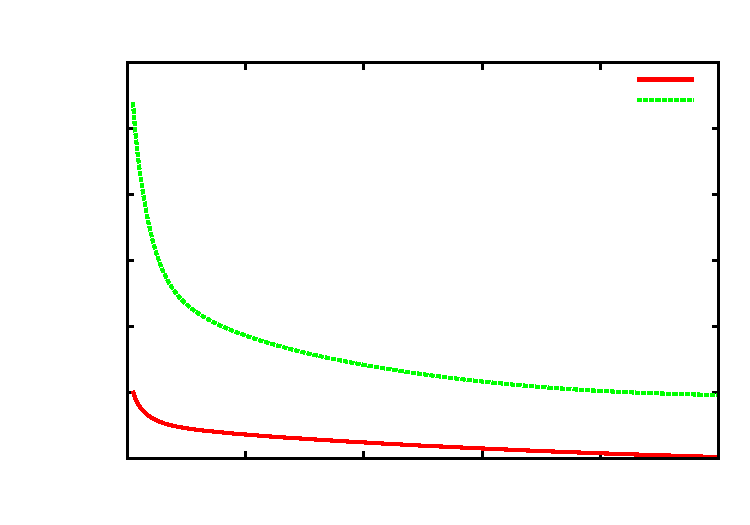
\includegraphics{figs/buffering}}%
    \gplfronttext
  \end{picture}%
\endgroup

  \caption{\label{buffering}This graph shows the advantage of using a buffered file writer over repeated calls to the printf() method. 
  The data was generated from a simulation using a 100x100 grid, but results will be similar for all grid sizes, since write time and computation
  time (neglecting overhead) both scale linearly with the number of cells.}
  \end{center}
  \end{figure} 

	 In Figure \ref{overhead} we attempt to quantify the overhead in our code. This is done by calculating the total time spent on each cell in a 
	 simulation, relative to the size of the simulation. With this metric, the code actually becomes `slower' for smaller simulations. This is 
	 because a significant fraction of the simulation time is being spent on finding arrays of neighbours and other `non essential' tasks. The graph
	 shows that our code only begins to run as efficiently as possible once grids of $\sim$100x100 are used, above which the simulation time scales
	 almost exactly as the number of cells (the flat part of Figure \ref{overhead}).\newline{}
	 
	 A `perfect' algorithm would spend the same amount of time on each cell regardless of grid size, but our code expends some effort on simplifying the problem 
	 at the start of a run by creating the neighbours array. This allows it to be slightly faster on large grids, but adds overhead which becomes non-negligible 
	 for small simulations.\newline{}
	 
  \begin{figure}[h]
  \begin{center}
  % GNUPLOT: LaTeX picture with Postscript
\begingroup
  \makeatletter
  \providecommand\color[2][]{%
    \GenericError{(gnuplot) \space\space\space\@spaces}{%
      Package color not loaded in conjunction with
      terminal option `colourtext'%
    }{See the gnuplot documentation for explanation.%
    }{Either use 'blacktext' in gnuplot or load the package
      color.sty in LaTeX.}%
    \renewcommand\color[2][]{}%
  }%
  \providecommand\includegraphics[2][]{%
    \GenericError{(gnuplot) \space\space\space\@spaces}{%
      Package graphicx or graphics not loaded%
    }{See the gnuplot documentation for explanation.%
    }{The gnuplot epslatex terminal needs graphicx.sty or graphics.sty.}%
    \renewcommand\includegraphics[2][]{}%
  }%
  \providecommand\rotatebox[2]{#2}%
  \@ifundefined{ifGPcolor}{%
    \newif\ifGPcolor
    \GPcolortrue
  }{}%
  \@ifundefined{ifGPblacktext}{%
    \newif\ifGPblacktext
    \GPblacktexttrue
  }{}%
  % define a \g@addto@macro without @ in the name:
  \let\gplgaddtomacro\g@addto@macro
  % define empty templates for all commands taking text:
  \gdef\gplbacktext{}%
  \gdef\gplfronttext{}%
  \makeatother
  \ifGPblacktext
    % no textcolor at all
    \def\colorrgb#1{}%
    \def\colorgray#1{}%
  \else
    % gray or color?
    \ifGPcolor
      \def\colorrgb#1{\color[rgb]{#1}}%
      \def\colorgray#1{\color[gray]{#1}}%
      \expandafter\def\csname LTw\endcsname{\color{white}}%
      \expandafter\def\csname LTb\endcsname{\color{black}}%
      \expandafter\def\csname LTa\endcsname{\color{black}}%
      \expandafter\def\csname LT0\endcsname{\color[rgb]{1,0,0}}%
      \expandafter\def\csname LT1\endcsname{\color[rgb]{0,1,0}}%
      \expandafter\def\csname LT2\endcsname{\color[rgb]{0,0,1}}%
      \expandafter\def\csname LT3\endcsname{\color[rgb]{1,0,1}}%
      \expandafter\def\csname LT4\endcsname{\color[rgb]{0,1,1}}%
      \expandafter\def\csname LT5\endcsname{\color[rgb]{1,1,0}}%
      \expandafter\def\csname LT6\endcsname{\color[rgb]{0,0,0}}%
      \expandafter\def\csname LT7\endcsname{\color[rgb]{1,0.3,0}}%
      \expandafter\def\csname LT8\endcsname{\color[rgb]{0.5,0.5,0.5}}%
    \else
      % gray
      \def\colorrgb#1{\color{black}}%
      \def\colorgray#1{\color[gray]{#1}}%
      \expandafter\def\csname LTw\endcsname{\color{white}}%
      \expandafter\def\csname LTb\endcsname{\color{black}}%
      \expandafter\def\csname LTa\endcsname{\color{black}}%
      \expandafter\def\csname LT0\endcsname{\color{black}}%
      \expandafter\def\csname LT1\endcsname{\color{black}}%
      \expandafter\def\csname LT2\endcsname{\color{black}}%
      \expandafter\def\csname LT3\endcsname{\color{black}}%
      \expandafter\def\csname LT4\endcsname{\color{black}}%
      \expandafter\def\csname LT5\endcsname{\color{black}}%
      \expandafter\def\csname LT6\endcsname{\color{black}}%
      \expandafter\def\csname LT7\endcsname{\color{black}}%
      \expandafter\def\csname LT8\endcsname{\color{black}}%
    \fi
  \fi
  \setlength{\unitlength}{0.0500bp}%
  \begin{picture}(7200.00,4536.00)%
    \gplgaddtomacro\gplbacktext{%
      \csname LTb\endcsname%
      \put(1100,640){\makebox(0,0)[r]{\strut{}-3.5}}%
      \put(1100,1111){\makebox(0,0)[r]{\strut{}-3.0}}%
      \put(1100,1582){\makebox(0,0)[r]{\strut{}-2.5}}%
      \put(1100,2053){\makebox(0,0)[r]{\strut{}-2.0}}%
      \put(1100,2523){\makebox(0,0)[r]{\strut{}-1.5}}%
      \put(1100,2994){\makebox(0,0)[r]{\strut{}-1.0}}%
      \put(1100,3465){\makebox(0,0)[r]{\strut{}-0.5}}%
      \put(1100,3936){\makebox(0,0)[r]{\strut{} 0.0}}%
      \put(1220,440){\makebox(0,0){\strut{} 0}}%
      \put(2167,440){\makebox(0,0){\strut{} 1}}%
      \put(3113,440){\makebox(0,0){\strut{} 2}}%
      \put(4060,440){\makebox(0,0){\strut{} 3}}%
      \put(5007,440){\makebox(0,0){\strut{} 4}}%
      \put(5953,440){\makebox(0,0){\strut{} 5}}%
      \put(6900,440){\makebox(0,0){\strut{} 6}}%
      \put(400,2288){\rotatebox{90}{\makebox(0,0){\strut{}log$_{10}$ Time/Cell [s]}}}%
      \put(4060,140){\makebox(0,0){\strut{}log$_{10}$ Number of Cells}}%
      \put(4060,4236){\makebox(0,0){\strut{}Run Time/Number of Cells vs. Number of Cells}}%
    }%
    \gplgaddtomacro\gplfronttext{%
      \csname LTb\endcsname%
      \put(5997,3773){\makebox(0,0)[r]{\strut{}Run Time/Number of Cells}}%
    }%
    \gplbacktext
    \put(0,0){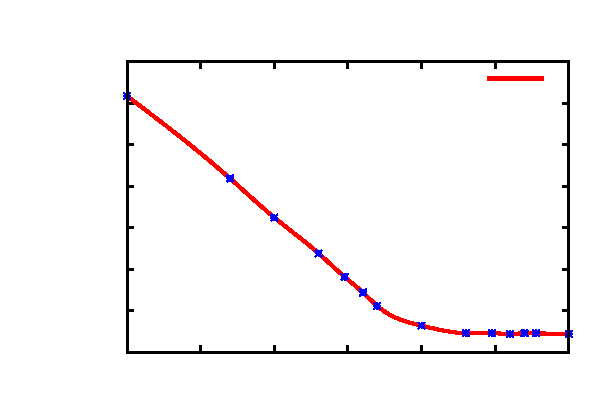
\includegraphics{figs/overhead}}%
    \gplfronttext
  \end{picture}%
\endgroup

  \caption{\label{overhead}This is a graph of total time spent on each cell, which shows that overheads such as array initialization
  take up a significant fraction of computation time with grids smaller than $\sim$100 by 100.}
  \end{center}
  \end{figure}
  
	 
   The main conclusion we reached in our testing is that output, espcially large amounts of plain text, is \emph{expensive}. The performance of
   the program could be dramatically increased by having the output in a more efficient format. This can be shown more simply just by running the 
   code with an output frequency of 20 timesteps compared with an output frequency of 2000 timesteps (a single output for a t=0..500, timestep=0.4
   simulation). This give run times of $\sim$38.0 and $\sim$31.5 seconds respectively, even with buffered output. This output then accounts for 
   $\sim$ 17\% of the computation time of a simulation, which obviously not ideal.  \newline{}

